\documentclass[12pt,a4paper]{ULBReport} %Template de rapport
\usepackage[utf8]{inputenc}
\graphicspath{ {./Pictures/} }
\sceau{Pictures/sceauULB.jpg}
\usepackage{multirow}
\usepackage{listings}
\usepackage{color} 
\usepackage{setspace} 
\usepackage{amsmath}
\usepackage{color}
\usepackage{hyperref}
\usepackage{biblatex}
\usepackage{floatrow}
\usepackage{graphicx}
\usepackage{float}
\usepackage{subcaption}


\addbibresource{biblio.bib}


\lstdefinelanguage{Python}{ 
numbers=left, 
numberstyle=\footnotesize, 
numbersep=1em, 
xleftmargin=1em, 
framextopmargin=2em, 
framexbottommargin=2em, 
showspaces=false, 
showtabs=false, 
showstringspaces=false, 
frame=l, 
tabsize=4, 
% Basic 
basicstyle=\ttfamily\small\setstretch{1}, 
backgroundcolor=\color{Background}, 
% Comments 
commentstyle=\color{Comments}\slshape, 
% Strings 
stringstyle=\color{Strings}, 
morecomment=[s][\color{Strings}]{"""}{"""}, 
morecomment=[s][\color{Strings}]{'''}{'''}, 
% keywords 
morekeywords={import,from,class,def,for,while,if,is,in,elif,else,not,and,or,print,break,continue,return,True,False,None,access,as,,del,except,exec,finally,global,import,lambda,pass,print,raise,try,assert}, 
keywordstyle={\color{Keywords}\bfseries}, 
% additional keywords 
morekeywords={[2]@invariant,pylab,numpy,np,scipy}, 
keywordstyle={[2]\color{Decorators}\slshape}, 
emph={self}, 
emphstyle={\color{self}\slshape}, 
% 
} 

\newcommand{\dd}[1]{\mathrm{d}#1}
\newcommand{\avec}[0]{
    \hspace{0.2cm}
    \text{avec :}
    \hspace{0.2cm}
}
\newcommand{\ou}[0]{
    \hspace{0.2cm}
    \text{d'où : }
    \hspace{0.2cm}
}
\newcommand{\et}[0]{
    \hspace{0.2cm}
    \text{et}
    \hspace{0.2cm}
}
\newcommand{\mtxt}[1]{
    \hspace{0.2cm}
    \text{#1}
}

%La Commande \TODO permet de mettre en rouge clairement ce qu'il reste à faire.
\newcommand{\TODO}[1]{
    \color{red}
    \textbf{TODO : } #1
    \color{black}
}

\begin{document}

\titleULB {
    title={Rapport : Design of a joint radar and communication system},
    studies={IRCI - BA3 Eléctronique et télécommunication},
    course ={ELEC-H311 : Signaux et systèmes de télécommunications},
    author={\textit{Auteurs:} \\ BOLLENGIER Alexis \\SCHEENAERTS Louis },
    date={\textbf{Année Académique :} \\ 2023 - 2024},
    teacher={\textit{Professeur : } \\ HORLIN François},
    logo={Pictures/logo-polytech.jpg},
    manyAuthor
}

%--------------------------------%

\chapter{Step 1: FMCW Signal}
\section {Génération et Caractérisation du \textit{Chirp FMCW}}

Dans cette première étape, l'objectif était la génération et la caractérisation d'un \textit{chirp FMCW}. Un seul \textit{chirp} de durée \( T \) a été utilisé, ce dernier a été obtenu en modulant une porteuse en fréquence (modulation de fréquence, FM) avec un message linéairement croissant sur le temps, représenté par une pente \( \beta = \frac{B}{T} \). La fréquence instantanée \( f_i(t) \) sur l'intervalle [0, T] est définie comme \( f_i(t) = \beta t \). La figure \ref{fig:fi_t_chirp} montre la fréquence instantanée en fonction du temps d'un seul \textit{chirp}.

\begin{figure}[H]
  \centering
  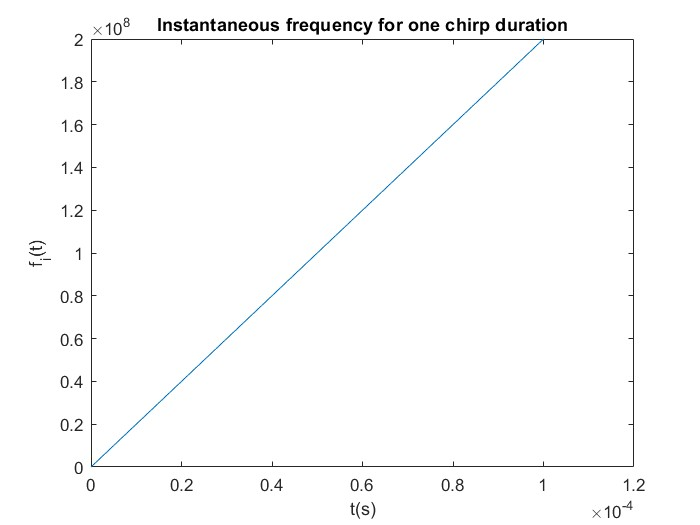
\includegraphics[scale = 0.25]{Pictures/one_chirp.jpg}
    \caption{\( f_i(t) \) pour un seul \textit{chirp} d'une durée de 0,4 ms }
    \label{fig:fi_t_chirp}
\end{figure}

Le signal transmis \( s(t) \) est modélisé par l'équation \ref{eq:s_transmis}.

\begin{equation} 
    s(t) = \cos(2\pi f_ct + \phi_i(t))
    \label{eq:s_transmis}
\end{equation}

où \( f_c \) est la fréquence porteuse et \( \phi_i(t) \) est la phase instantanée obtenue en intégrant \( f_i(t) \).

L'intégration de \( f_i(t) \) pour obtenir \( \phi_i(t) \) est formulée par l'équation \ref{eq:phi_inst}.

% Expression pour la phase instantanée
\begin{equation}
    \phi_i(t) = 2\pi \int_{0}^{t} f_i(u) \, du
    \label{eq:phi_inst}
\end{equation}

% Explication de l'intégrale
% Ici, \phi_i(t) représente la phase instantanée du signal FMCW, 
% calculée comme l'intégrale cumulée de la fréquence instantanée \( f_i(u) \) 
% sur l'intervalle [0, t]. Cela capture l'évolution de la phase du signal 
% en fonction du temps.

L'équation \ref{eq:signal_bb} permet la génération du signal en bande de base \( e^{j\phi_i(t)} \) 

\begin{equation}
    \text{signal en bande de base} = e^{(j \phi_i)}
    \label{eq:signal_bb}
\end{equation}

Ici, la fréquence instantanée \( f_i(t) \) est intégrée pour obtenir la phase instantanée \( \phi_i(t) \). Le signal en bande de base \( e^{j\phi_i(t)} \) est ainsi généré, représentant un \textit{chirp FMCW}.

En considérant le cas où le \textit{chirp} est répété indéfiniment sur le temps, similaire à un signal \textit{FMCW}, sa réponse en fréquence est échantillonnée à la cadence de répétition. Les conclusions tirées pour un seul \textit{chirp} dans cette étape sont donc généralisables à l'ensemble du signal \textit{FMCW}.

\section {Représentation du Signal en Temps et en Fréquence}

Cette génération de \textit{chirp} a été implantée en utilisant les paramètres suivants :
\begin{itemize}
  \item Plage de fréquence : \( B = 200 \, \text{MHz} \)
  \item Durée du \textit{chirp} : \( T = 0.2 \, \text{ms} \)
  \item Fréquence d'échantillonnage : \( F_s = 512 \, \text{MHz} \)
  \item Nombre d'échantillons : \( 2^{18} \)
\end{itemize}

%Le code Python associé permet de générer la fréquence instantanée \( f_i(t) \) en fonction du temps sur une durée de \textit{chirp}. Il permet aussi de produire le signal transmis en bande de base \( e^{j\phi_i(t)} \).

Les résultats ont été illustrés graphiquement, avec la partie réelle du signal en bande de base agrandie sur l'intervalle \( T \in [0; 4 \times 10^{-6}]\) dans la  sous-figure \ref{subfig:s_BB_zoom}, et la partie réelle du signal en bande de base sur l'intervalle \( T \in [0; 2T]\) dans la sous-figure \ref{subfig:s_BB_entier}.

\begin{figure}[H]
  \centering
  \begin{subfigure}[b]{0.45\textwidth}
    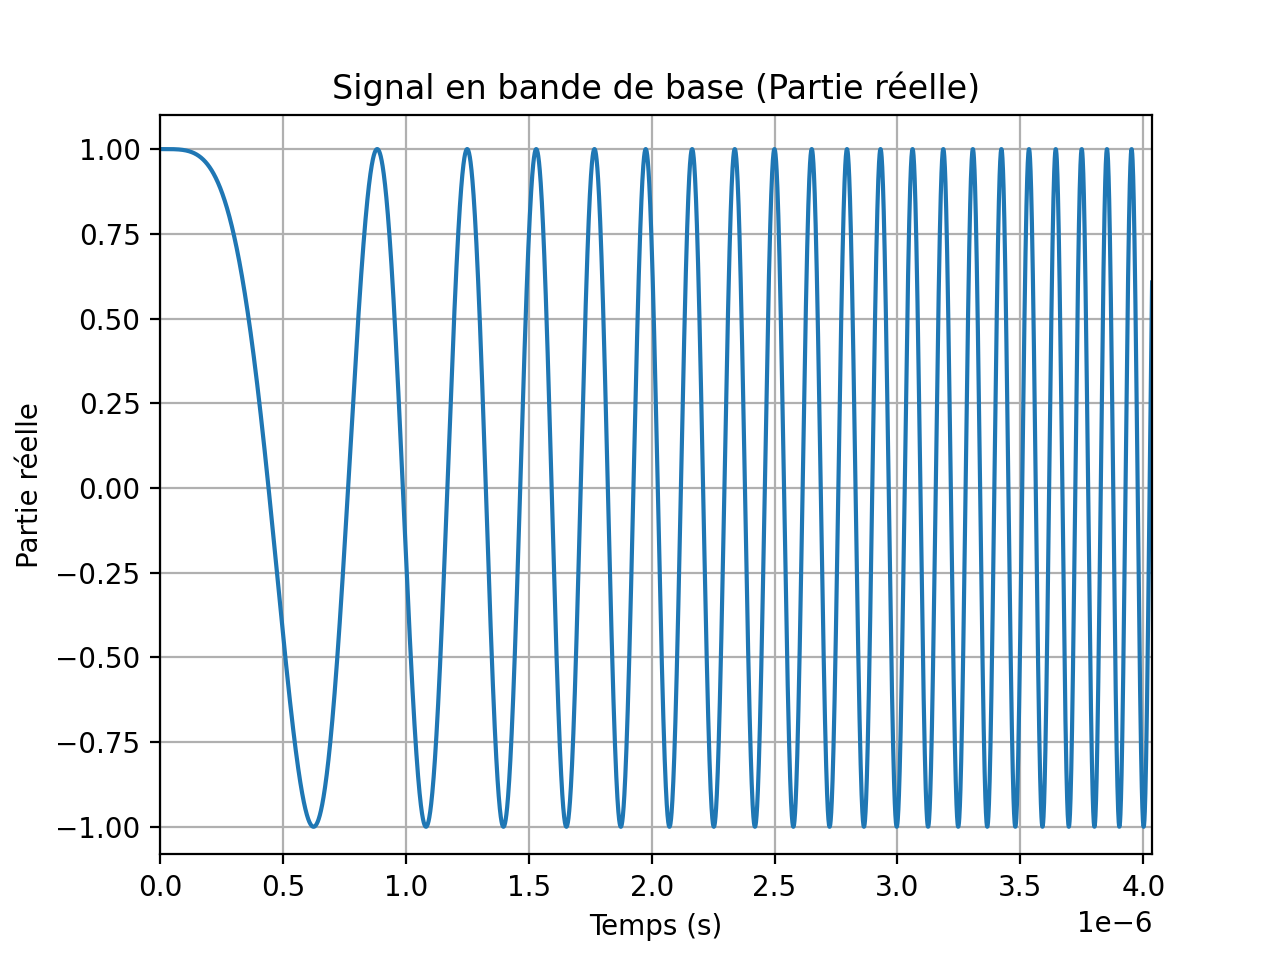
\includegraphics[width=\textwidth]{Pictures/BNDBR_SST.png}
    \caption{Partie réelle du signal en bande de base agrandie sur \(T \in [0; 4 \times 10^{-6}]\).}
    \label{subfig:s_BB_zoom}
  \end{subfigure}
  \hfill
  \begin{subfigure}[b]{0.45\textwidth}
    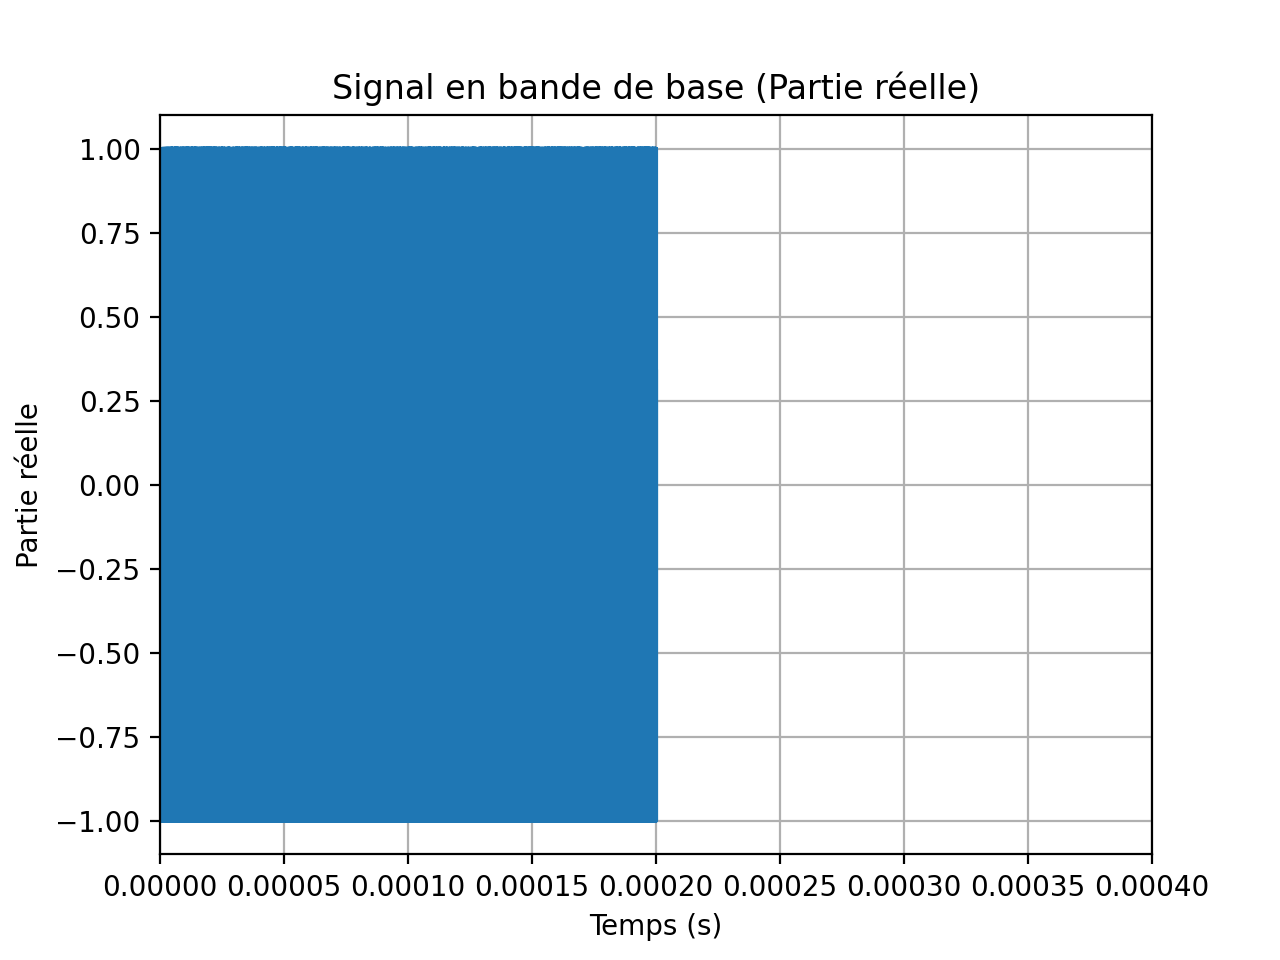
\includegraphics[width=\textwidth]{Pictures/BNDBR_SST(1).png}
    \caption{Partie réelle du signal en bande de base \(T \in [0; 2T]\).}
    \label{subfig:s_BB_entier}
  \end{subfigure}
  \caption{Représentation du \textit{chirp} dans le domaine temporel}
  \label{fig:chirp_temp}
\end{figure}

\section {Analyse Fréquentielle du Signal}

En effectuant la transformée de Fourier du signal, il est possible d'obtenir le spectre de fréquence en bande de base. La figure \ref{fig:spectre_bbs} représente l'amplitude du spectre de fréquence pour deux valeurs de $T$ différentes.

\begin{figure}[H]
  \centering
  \begin{subfigure}[b]{0.45\textwidth}
    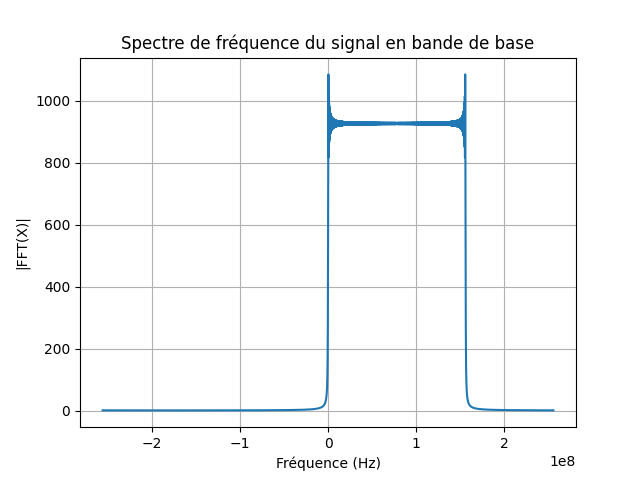
\includegraphics[width=\textwidth]{Pictures/SPCTR_SST.png}
    \caption{Spectre de fréquence du signal en bande de base pour $T=0.4$ms}
  \end{subfigure}
  \hfill
  \begin{subfigure}[b]{0.45\textwidth}
    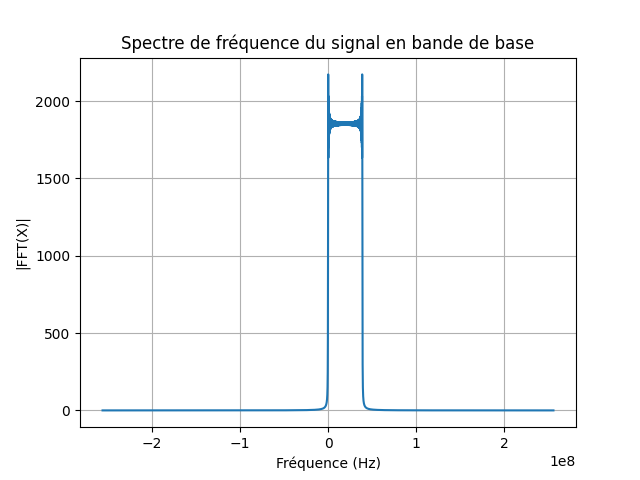
\includegraphics[width=\textwidth]{Pictures/SPCTR_SST(1).png}
    \caption{Spectre de fréquence du signal en bande de base pour $T=0.1$ms}
  \end{subfigure}
  \caption{Spectre de fréquence du signal en bande de base avec deux valeurs de $T$.}
  \label{fig:spectre_bbs}
\end{figure}

\section {Discussion de l'Impact de la Durée du \textit{Chirp} sur la Bande Passante}

Comme le montre la figure \ref{fig:spectre_bbs}, la durée du \textit{chirp} ($T$)  influence la plage de fréquences couvertes et donc la résolution en distance. Une durée plus longue permet une couverture fréquentielle plus étendue, améliorant la résolution en distance. Cependant, cela augmente également la consommation de bande passante, ce qui peut être limitant dans certaines applications.



\chapter{Step 2: Radar processing}
\section{Generation d'une Suite de \textit{Chirps}}

Il est possible de répéter la génération d'un \textit{chirp} $K$ fois en utilisant l'équation \ref{eq:t_all_chirps} comme base de temps afin d'obtenir une suite de \textit{chirps} qui va composer le signal qui sera envoyé.

\begin{equation}
    t = kT + t^\prime
    \label{eq:t_all_chirps}
\end{equation}

 Avec $t^\prime$ qui est le temps par \textit{chirp} (\(t^\prime \in [0,T]\)) et k qui est le \textit{chirp} qui est généré (\(k \in [0,K-1]\)). Dans la simulation, le paramètre $K$ vaut 256.

\section{Simulation des \textit{Chirps} Reçues}

Après avoir été émis, le signal va être réfléchis par les cibles et revenir avec un certain décalage temporel du à la distance et fréquentiel du à la vitesse de la cible. Dix cibles aléatoires ont été simulées dans le code fournit avec ce laboratoire. La figure \ref{fig:all_chirp} montre le signal qui est émis et les signaux qui sont réfléchis par les différentes cibles. Étant donné le fait que les cibles sont dans la voisinage du radar, les signaux réfléchis sont très proches des signaux émis. La figure \ref{fig:all_chirp_zoom} est un agrandissement de la figure \ref{fig:all_chirp} qui permet de distinguer les différents signaux réfléchis. 

\begin{figure}[H]
  \centering
  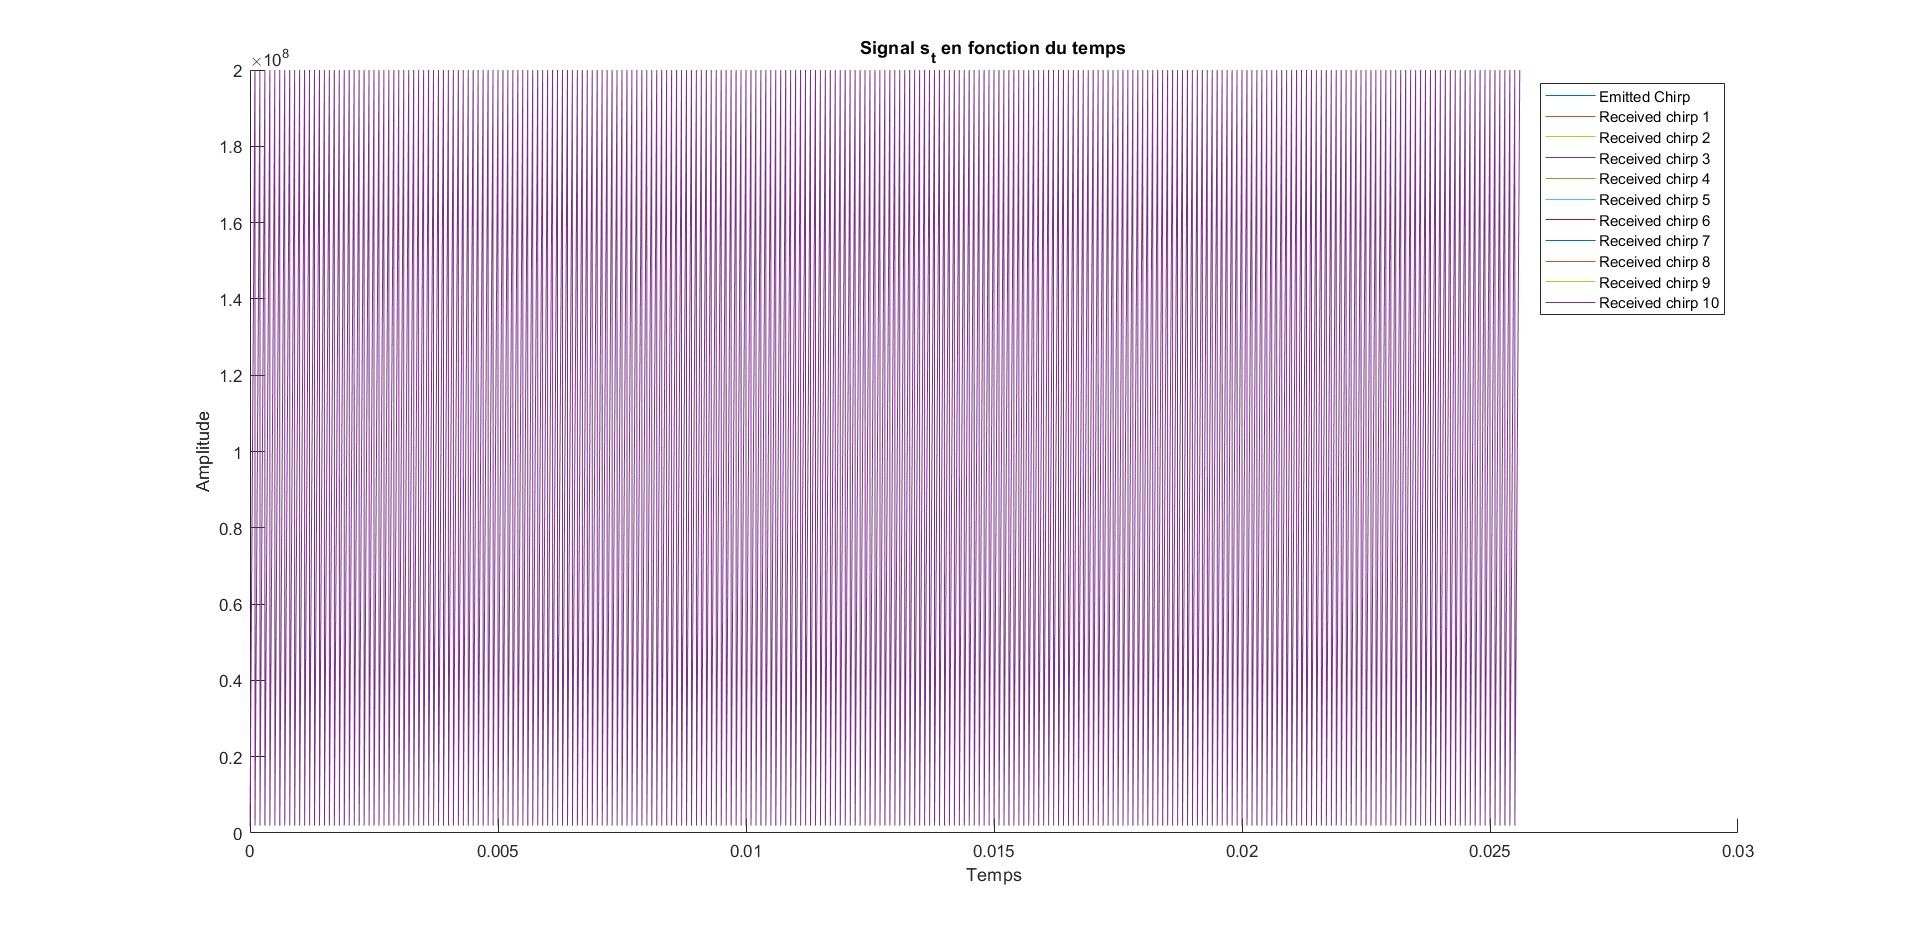
\includegraphics[scale = 0.2]{Pictures/multiple_target.jpg}  \caption{Vue d'ensemble des \textit{chirps} émis et reçus}
  \label{fig:all_chirp}
\end{figure}

\begin{figure}[H]
  \centering
  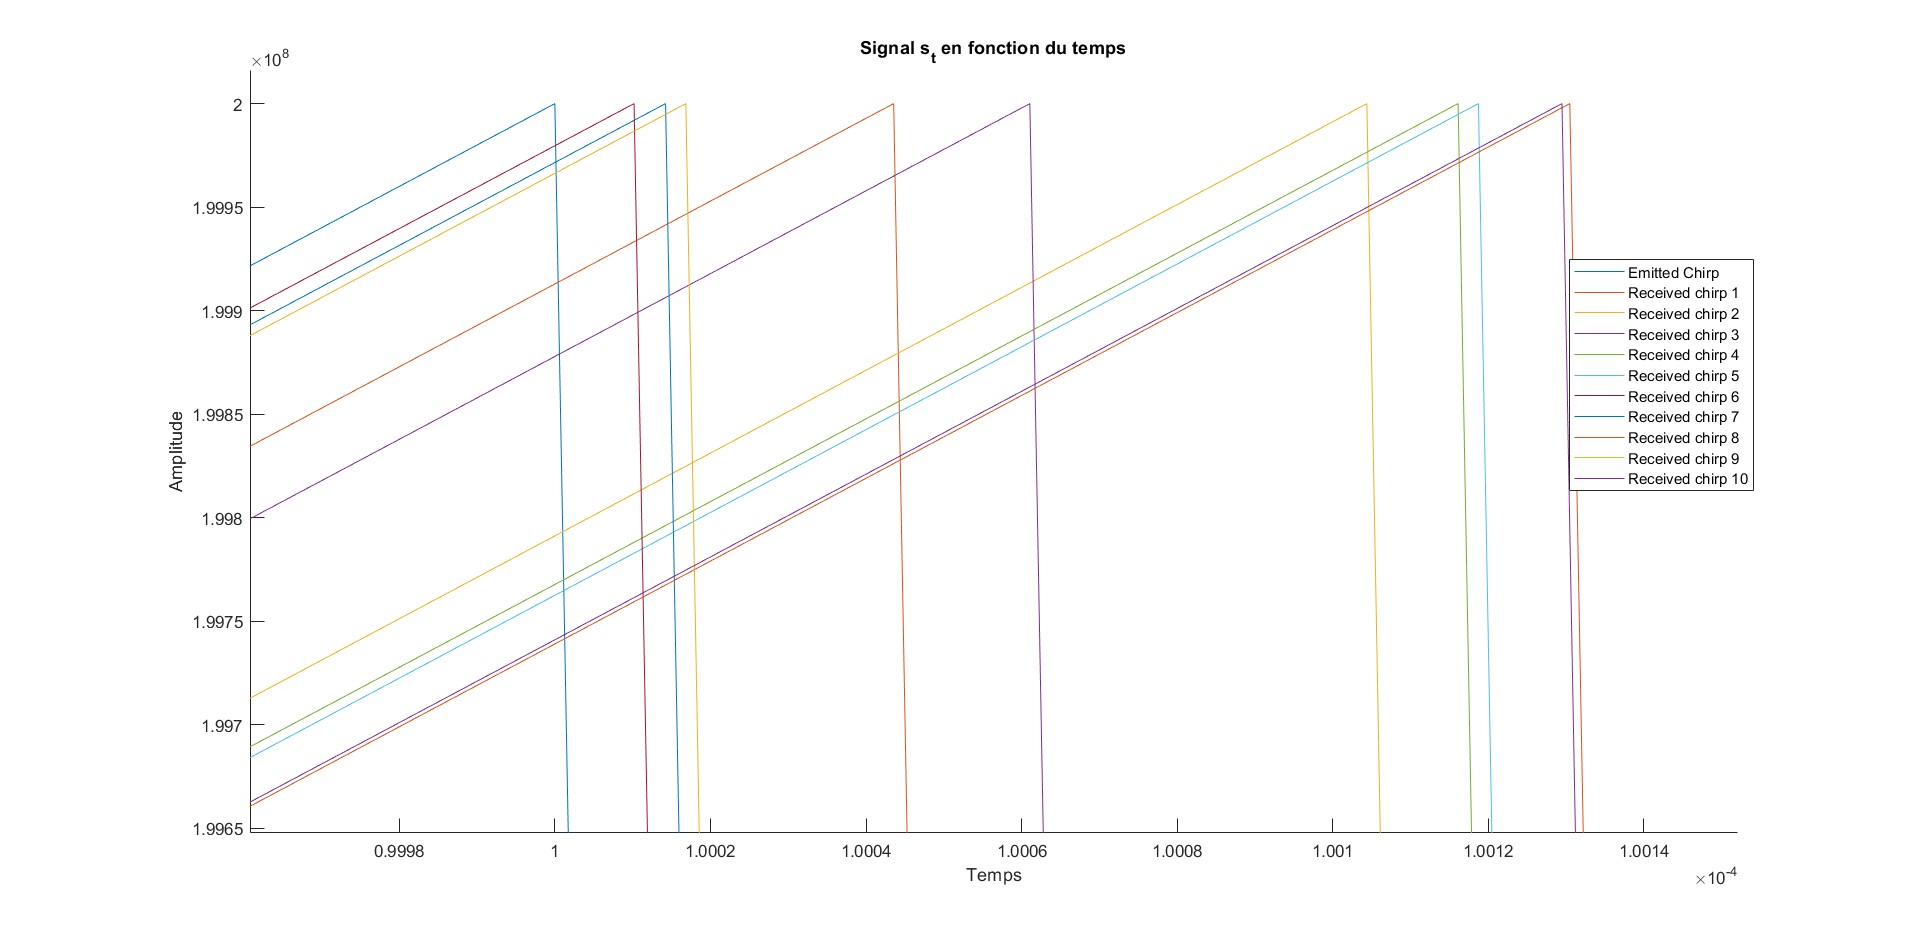
\includegraphics[scale = 0.2]{Pictures/multiple_target_zoom.jpg}  \caption{Vue rapprochée des \textit{chirps} émis et reçus}
  \label{fig:all_chirp_zoom}
\end{figure}


\section{\textit{Range Doppler Map}}

\subsection{Génération des Signaux Radar}

Les signaux radar sont générés selon deux méthodes distinctes : la Figure 4 et l'équation 16 des principes du radar FMCW \footnote{Fig 4 et eq (16) du pdf RadarFMCW du cours}. Chaque méthode est appliquée à chaque \textit{chirp} et le résultat est stocké dans une matrice NxK. Les matrices résultantes, \(NxK^{(\text{Fig.4})}\) et \(NxK^{(\text{Eq.16})}\), représentent les signaux générés pour chaque échantillon de fréquence Doppler \(K\) et chaque instant de temps \(N\). 

\subsection {Obtention de la RDM}

La RDM est obtenue grâce à plusieurs transformée de Fourier. La première transformée se fait sur chaque colonne de la matrice NxK. La deuxième se fait sur les lignes de la matrice obtenu après la première transformée. La dernière est une transformée de Fourrier 2D. L'étape finale consiste à sommer les RDM obtenues pour chaque cibles pour n'en avoir qu'une seule au final. La figure \ref{fig:RDM_2_ways} montre les RDM obtenues selon les deux méthodes. Elle permet aussi de montrer qu'il n'y a pas de différences entre l'utilisation de l'équation 16 ou de la figure 4. 

\begin{figure}[H]
  \centering
  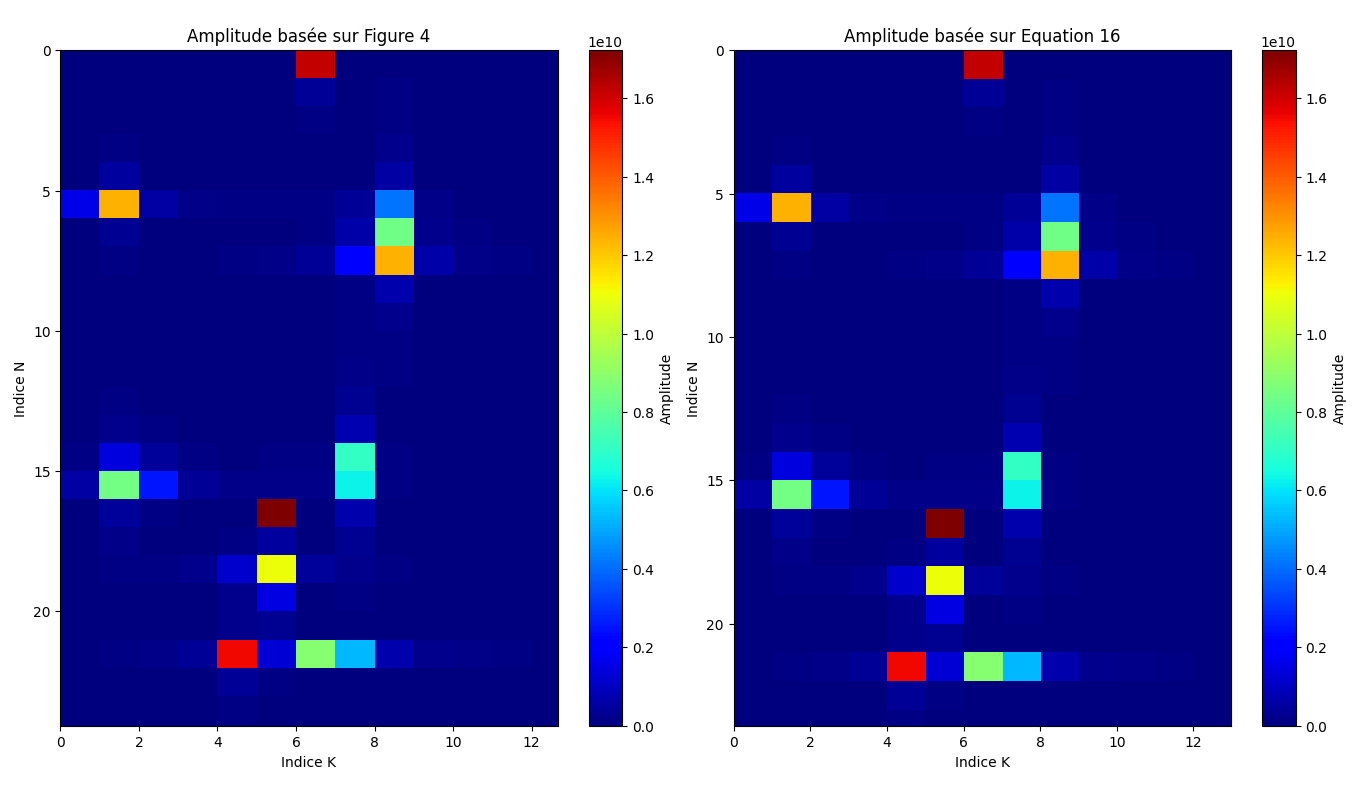
\includegraphics[scale =0.4]{Pictures/RDM_P_SST.png}
    \caption{RDM obtenues par deux moyens différents}
    \label{fig:RDM_2_ways}
\end{figure}

Sur base de la figure \ref{fig:RDM_2_ways} et des définitions des résolutions ( $\Delta R_0 = \frac{c}{2B} = 0,75 m$ et $\Delta v = \frac{c}{2KTF_c} = 0.24 m/s$), il est possible de retrouver approximativement les positions et vitesses des différentes cibles en multipliant les indices K et N par leurs résolutions. Le tableau \ref{tab:results_calc_RDM} montre les résultats ainsi calculés. Il est important de noter que seul des vitesses et des distances positives ont été prises en compte dans le cadre de ce projet.  

\begin{table}[H]
    \centering
    \begin{tabular}{|c|c|c|c|c|c|}
    \hline
    \rowcolor[gray]{0.90} $R_0$ [m] &  $v$ [m/s] &  $N$ [ ] &  $K$ [ ] & $R_{0_{estimé}}$ [m] &  $v_{estimé}$ [m/s]  \\\hline
 5,41  & 1,88 & 7  & 8 & 5,25  & 1,92 \\\hline
 11,11 & 0,33 & 15 & 1 & 11,25 & 0,24 \\\hline
 12,10 & 1,23 & 16 & 5 & 13,50 & 1,20 \\\hline
 15,96 & 1,01 & 21 & 4 & 15,75 & 0,96 \\\hline
 4,22  & 1,90 & 6  & 8 & 4,50  & 1,92 \\\hline
 13,80 & 1,16 & 18 & 5 & 13.50 & 1,20 \\\hline
 10,94 & 1,68 & 14 & 7 & 10,50 & 1,68 \\\hline
 3,65  & 0,18 & 5  & 1 & 3,75  & 0,24 \\\hline
 0,10  & 1,47 & 0  & 6 & 0,00  & 1,44 \\\hline
 15,89 & 1,57 & 21 & 6 & 15,75 & 1,44 \\\hline
    \end{tabular}
    \caption{vitesses réelles, vitesses mesurées et indices sur la RDM}
    \label{tab:results_calc_RDM}
\end{table}

\subsection{Discussion sur le Choix des Paramètres}

Afin de discuter de la pertinence des paramètres choisis étant donné la situation qui est analysée, il faut calculer la portée maximale estimée $\left(\frac{cTF_s}{2B}\right)$  ainsi que l'intervalle d'estimation de la vitesse $\left(\frac{c}{4TF_c}\right)$. Ces deux valeurs valent respectivement 150 m et 31,25 m/s avec les paramètres choisis. En sachant que la distance maximale est de 20 m et que la vitesse maximale est de 2 m/s, il n'y a que 13,3\% de la portée maximale qui est exploitée et seulement 6,4\% de l'intervalle de vitesse qui est exploité. Ceci ainsi que le calul des résolutions fait au point précédent montre que les paramètres du radar ne sont pas choisis de manière optimal pour l'application visée. En augmentant $B$ et $F_c$, il serait possible d'avoir de meilleurs résolutions ainsi qu'une meilleur utilisation de la RDM. 


\chapter{Step 3: Radar performance analysis}
\section{Ajout du Bruit Blanc Gaussien }
Le bruit blanc gaussien est un type de bruit aléatoire dont les échantillons sont tirés d'une distribution gaussienne c'est à dire, un bruit aléatoire dont les composantes réelles et imaginaires suivent une distribution normale. Ici, une moyenne nulle et un écart type de 1 ont été considérés.
Dans le code python celui ci est ajouté via la fonction \texttt{add\_awgn}.

En calculant le Rapport Signal sur Bruit (SNR) pour différentes valeurs, une atténuation des amplitudes des signaux reçus avec bruit devient visible, due au fait que la puissance du bruit ajouté rend plus difficile la distinction entre le bruit et le signal. Un faible SNR engendre une grande puissance de bruit (\ref{eq:p_bruit}), compliquant ainsi la distinction entre signal et bruit. De plus, l'ajout d'un SNR négatif conduit à un \textit{SNR\_linear} < 1, ce qui signifie que $P_{\text{bruit}} > P_{\text{signal}}$. Le radar FMCW détecte alors des cibles fantômes et atténue l'amplitude des signaux réels. Ceci s'illustre bien sur la comparaison des RDM qui est faite sur la figure \ref{fig:rdm_wn} pour différents valeurs de SNR.

\begin{figure}[H]
    \centering
    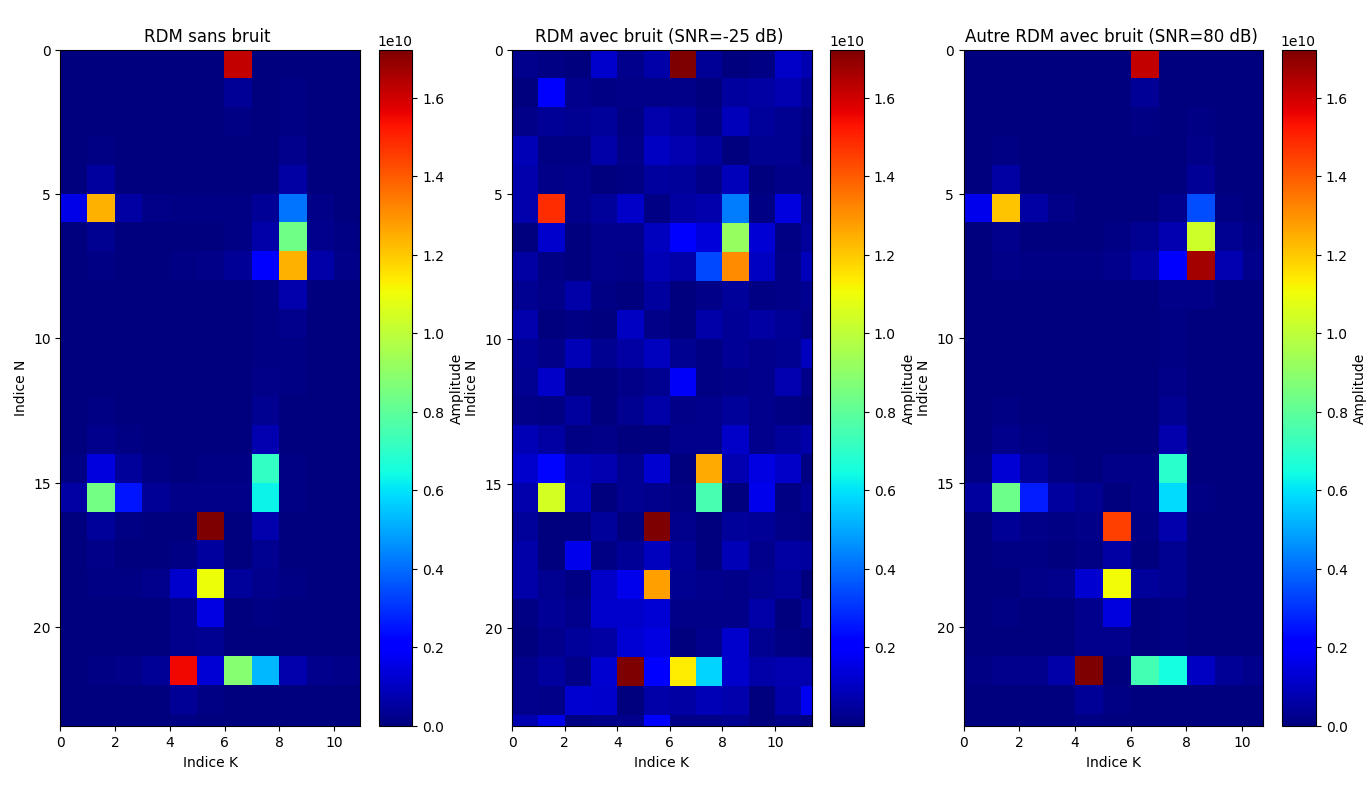
\includegraphics[width=0.77\textwidth]{Pictures/RDM_WITH_WITHOUT_SST_P.png}
    \caption{Comparaison entre RDM avec et sans bruit pour différentes valeurs de SNR}
    \label{fig:rdm_wn}
\end{figure}
\section{Detection des Cibles et Courbe ROC}
 
\subsection{\textit{True Positive Rate} (TPR) et \textit{False Positive Rate} (FPR)}

L'axe des abscisses dans la courbe ROC représente le FPR , également appelé taux de faux positifs. C'est la proportion d'échantillons de la classe négative qui sont incorrectement classés comme positifs par le modèle. Mathématiquement, le FPR est défini par l'équation \ref{eq:FPR}.

\begin{equation}
    FPR = \frac{\text{False Positives}}{\text{False Positives} + \text{True Negatives}}
    \label{eq:FPR}
\end{equation}


L'axe des ordonnées dans la courbe ROC représente le TPR  ou la sensibilité. Il s'agit de la proportion d'échantillons de la classe positive correctement classés comme positifs par le modèle. Le TPR est défini par l'quation \ref{eq:TPR}.

\begin{equation}
    TPR = \frac{\text{True Positives}}{\text{True Positives} + \text{False Negatives}}
    \label{eq:TPR}
\end{equation}

Maintenant, le lien avec la fonction \texttt{detect\_targets} est le suivant : la fonction génère une matrice booléenne (\texttt{binary\_map}) en appliquant un seuil à la RDM. Cette matrice est utilisée pour calculer le FPR et le TPR dans le contexte de la courbe ROC. Les vrais positifs et les faux positifs sont déterminés en comparant la résultante avec les véritables états de présence de cibles. Mathématiquement, la fonction \texttt{detect\_targets} peut être réprésenté:
\[
binary\_map=\begin{cases} 
True & \text{si } \text{{rdm > thresholds}} \\
False & \text{sinon}
\end{cases}
\]
\subsection{Courbe ROC }

La courbe ROC  est un outil essentiel pour évaluer la performance du radar \textit{FMCW} dans différents scénarios de bruit. Cette courbe illustre graphiquement la relation entre les taux de faux positifs (FPR) et de vrais positifs (TPR) en fonction des seuils de détection. Elle est calculée en utilisant la RDM sans bruit comme référence et en appliquant des seuils aux RDM avec bruit et ce pour différents niveaux de bruits.

Le graphe ROC, basé sur différentes valeurs de SNR, est présenté dans la figure \ref{fig:roc}. Il démontre la performance du radar pour chaque scénario de bruit, indiquant le compromis entre le TPR et le FPR. La ligne en pointillés représente le résultat attendu pour un modèle aléatoire.

\begin{figure}[H]
    \centering
    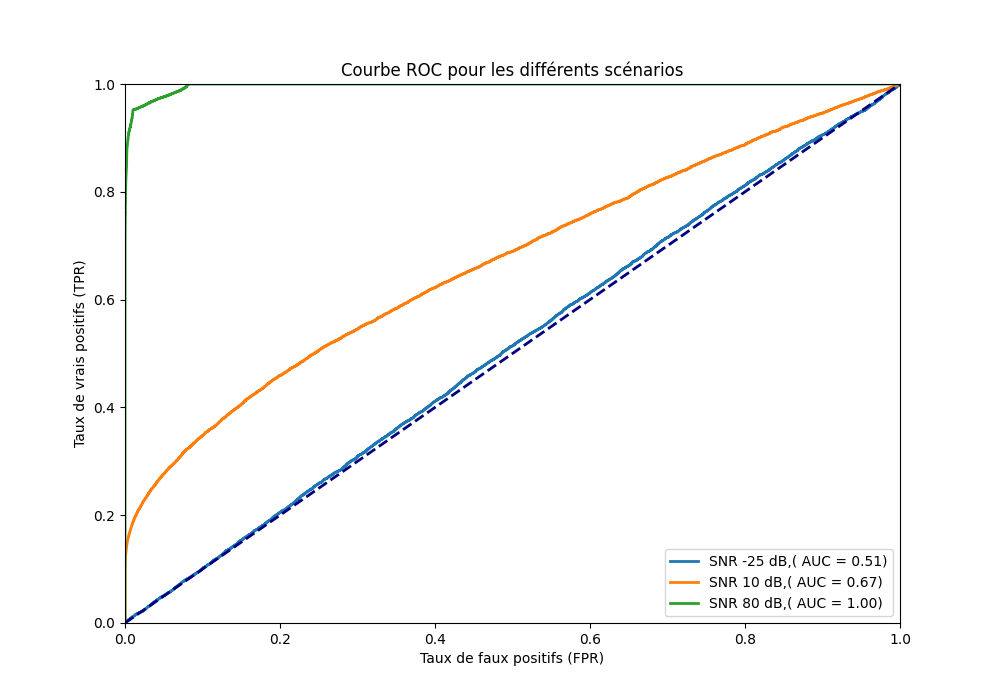
\includegraphics[width=0.8 \textwidth]{Pictures/ROC_SST_P.png}
    \caption{Courbe ROC pour les différents niveaux de bruits.}
    \label{fig:roc}
\end{figure}

L'aire sous la courbe (AUC) est calculée pour chaque valeur de SNR et est indiquée dans la légende du graphe. Une AUC proche de 1 indique une excellente performance, tandis qu'une valeur proche de 0.5 suggère une performance aléatoire.\\
\textbf{Discussion des valeurs des SNR}\\
Il est intéressant de voir que des valeurs de SNR plus élevées conduisent généralement à des AUC plus grandes, indiquant une meilleure capacité du radar à discriminer entre les cibles réelles et le bruit. Cela met en évidence l'importance des valeurs de SNR dans l'efficacité du radar en conditions réelles.

\chapter{Visit IMEC}
\section{Paramètres des Radars en Fonction de l'Application Visée}

Les distances et vitesses qui doivent être mesurées vont déterminer les paramètres du radar comme indiqué précédemment. Un autre point qui va influencer les paramètres du radar est la taille de l'émetteur et du récepteur. Plus une antenne est petite, plus la longueur d'onde qu'elle émet est petite et donc plus sa fréquence d'émission est grande.   
\section{Estimation des Angles d'Arrivées}

Afin d'estimer les angles d'arrivées (élévation et azimuth), il est nécessaire d'utiliser un réseau d'antenne tant à la réception qu'à l'émission. Les antennes émettrices vont chacune produire une fréquence orthogonale par rapport aux fréquences des autres antennes afin que les antennes réceptrices puissent identifier de quelle antenne émettrice un signal provient. La disposition spatiale des réseaux d'antenne fait que chaque antenne réceptrice recevra des signaux légèrement différents de chaque antenne émettrice. Il est donc possible de créer un réseau virtuel d'antenne afin d'avoir une bonne résolution angulaire. Une FFT supplémentaire sur le réseau virtuel d'antenne permet d'avoir une estimation  des deux angles. 
\section{Précision du Modèle Dévellopé et Différences Principales avec une Implémentation Réelle}

Le modèle dévellopé dans ce projet manque de précisions car la seule non-idéalité qui est prise en compte est le bruit thermique. En réalité, il existe d'autres sources de non-idéalités qui peuvent provenir du \textit{Hardware} comme le bruit de quantification et les non-linéarités d'un amplificateur opérationnel en saturation ou de l'environnement comme une cible fantôme ou des \textit{sidelobes}. Le bruit de quantification peut être réduit en augmentant le nombre de \textit{Bits} du quantifieur mais il faut que l'application le permette. Il est aussi possible d'avoir des ampli-op qui ont bonne linéarité dans la gamme de fréquence qui est prévu pour l'application. 
\section{Capacitées Actuelles et Evolutions Envisagées}

Dans l'état actuel, il est possible d'avoir des radars qui travaillent avec des fréquences porteuses de l'ordre de la centaine de GHz pour un $B$ de l'ordre de 10 GHz. Ceci permet d'avoir une résolution de plus ou moins 1.5cm à courte distance. Il est aussi possible de coupler les données obtenues par un radar \textit{FMCW} avec un algorithme de \textit{Machine Learning} afin de faire de la reconnaissance de \textit{pattern}. Les évolutions envisagées sont d'aller encore plus loin dans la miniaturisation des antennes et donc encore plus haut dans les fréquences mais aussi de développer des algorithmes de \textit{Machine Learning} plus complexes afin de reconnaître des \textit{patterns} plus compliqués.   

\begin{appendices}
\chapter{Puissance}

 \section{Signal Quelconque}
 
La puissance du signal (\(P_{\text{signal}}\)) est une mesure de l'énergie contenue dans le signal radar complexe. Elle est calculée en prenant la moyenne de la norme au carré de chaque échantillon du signal, comme indiqué par l'équation \ref{eq:P_signal} :

\begin{equation}
    P_{\text{signal}} = \frac{1}{N} \sum_{i=1}^{N} |x_i|^2
    \label{eq:P_signal}
\end{equation}

Ici, \(N\) représente le nombre total d'échantillons du signal radar complexe.\\

\section{\textit{Signal to Noise Ratio } (SNR)}

Le Rapport Signal sur Bruit (\textit{SNR}) en décibels est défini comme le rapport de la puissance du signal (\(P_{\text{signal}}\)) à la puissance du bruit (\(P_{\text{bruit}}\)), comme formulé par l'équation \ref{eq:SNR_db} :

\begin{equation}
    \text{SNR(dB)} = 10 \cdot \log_{10} \left( \frac{P_{\text{signal}}}{P_{\text{bruit}}} \right)
    \label{eq:SNR_db}
\end{equation}

\section{Puissance du bruit}

La puissance du bruit (\(P_{\text{bruit}}\)) est déduite de \ref{eq:SNR_db} et on obtiens :

\begin{equation}
    P_{\text{bruit}} = \frac{P_{\text{signal}}}{10^{(\text{SNR(dB)}/10)}}
    \label{eq:p_bruit}
\end{equation}
Ensuite, le bruit est calculé comme ci dessous:
\begin{equation}
    \text{Bruit} = \sqrt{\frac{P_{\text{bruit}}}{2}} \left(\mathcal{N}(0, 1) + j \cdot \mathcal{N}(0, 1)\right)
    \label{eq:bruit_blanc}
\end{equation}

La racine carrée de la moitié de la puissance du bruit est utilisée pour ajuster l'amplitude du bruit. Cela garantit que la variance du bruit est conforme à la puissance du bruit spécifiée.
\(\mathcal{N}(0, 1)\) représente un échantillon aléatoire tiré d'une distribution normale standard pour la partie réelle et imaginaire du bruit. Cela introduit une composante aléatoire qui caractérise le bruit blanc additif Gaussien

En combinant la partie réelle et imaginaire avec l'ajustement d'amplitude, l'équation génère un bruit blanc gaussien complexe qui peut être additionné\footnote{car on parle bien de bruit blanc \textbf{additif} Gaussien} au signal radar d'origine.\\
\section{Detection des Cibles et Courbe ROC}
 
\subsection{\textit{True Positive Rate} (TPR) et \textit{False Positive Rate} (FPR)}

L'axe des abscisses dans la courbe ROC représente le FPR , également appelé taux de faux positifs. C'est la proportion d'échantillons de la classe négative qui sont incorrectement classés comme positifs par le modèle. Mathématiquement, le FPR est défini par l'équation \ref{eq:FPR}.

\begin{equation}
    FPR = \frac{\text{False Positives}}{\text{False Positives} + \text{True Negatives}}
    \label{eq:FPR}
\end{equation}


L'axe des ordonnées dans la courbe ROC représente le TPR  ou la sensibilité. Il s'agit de la proportion d'échantillons de la classe positive correctement classés comme positifs par le modèle. Le TPR est défini par l'quation \ref{eq:TPR}.

\begin{equation}
    TPR = \frac{\text{True Positives}}{\text{True Positives} + \text{False Negatives}}
    \label{eq:TPR}
\end{equation}

Maintenant, le lien avec la fonction \texttt{detect\_targets} est le suivant : la fonction génère une matrice booléenne (\texttt{binary\_map}) en appliquant un seuil à la RDM. Cette matrice est utilisée pour calculer le FPR et le TPR dans le contexte de la courbe ROC. Les vrais positifs et les faux positifs sont déterminés en comparant la résultante avec les véritables états de présence de cibles. Mathématiquement, la fonction \texttt{detect\_targets} peut être réprésenté:
\[
binary\_map=\begin{cases} 
True & \text{si } \text{{rdm > thresholds}} \\
False & \text{sinon}
\end{cases}
\]
\subsection{Courbe ROC }

La courbe ROC  est un outil essentiel pour évaluer la performance du radar \textit{FMCW} dans différents scénarios de bruit. Cette courbe illustre graphiquement la relation entre les taux de faux positifs (FPR) et de vrais positifs (TPR) en fonction des seuils de détection. Elle est calculée en utilisant la RDM sans bruit comme référence et en appliquant des seuils aux RDM avec bruit et ce pour différents niveaux de bruits.

Le graphe ROC, basé sur différentes valeurs de SNR, est présenté dans la figure \ref{fig:roc}. Il démontre la performance du radar pour chaque scénario de bruit, indiquant le compromis entre le TPR et le FPR. La ligne en pointillés représente le résultat attendu pour un modèle aléatoire.

\begin{figure}[H]
    \centering
    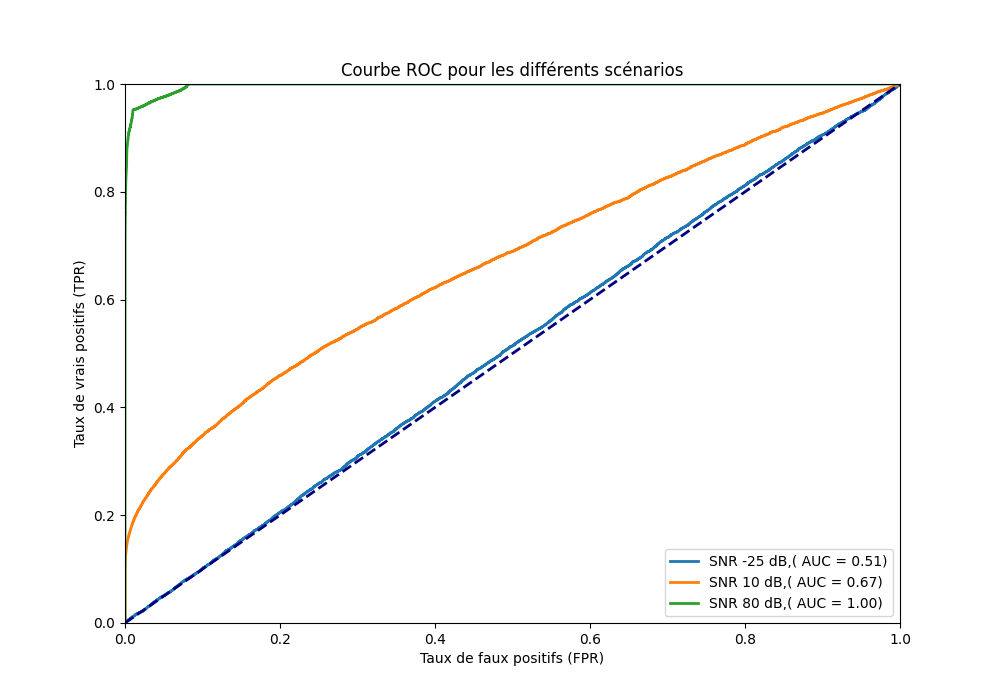
\includegraphics[width=0.8 \textwidth]{Pictures/ROC_SST_P.png}
    \caption{Courbe ROC pour les différents niveaux de bruits.}
    \label{fig:roc}
\end{figure}

L'aire sous la courbe (AUC) est calculée pour chaque valeur de SNR et est indiquée dans la légende du graphe. Une AUC proche de 1 indique une excellente performance, tandis qu'une valeur proche de 0.5 suggère une performance aléatoire.\\
\textbf{Discussion des valeurs des SNR}\\
Il est intéressant de voir que des valeurs de SNR plus élevées conduisent généralement à des AUC plus grandes, indiquant une meilleure capacité du radar à discriminer entre les cibles réelles et le bruit. Cela met en évidence l'importance des valeurs de SNR dans l'efficacité du radar en conditions réelles.

\end{appendices}
\end{document}
